% Give an introduction to the situational sketch and model system
% Present the communication model
% Argument design choices

We created a model for our bridge to account for the sequenced actions necessary to open and close the bridge in a safe manner. The model and its components are displayed in figure \ref{fig:model}. 
%--------------- Image of the model------------

\begin{figure}[!h]
\centering
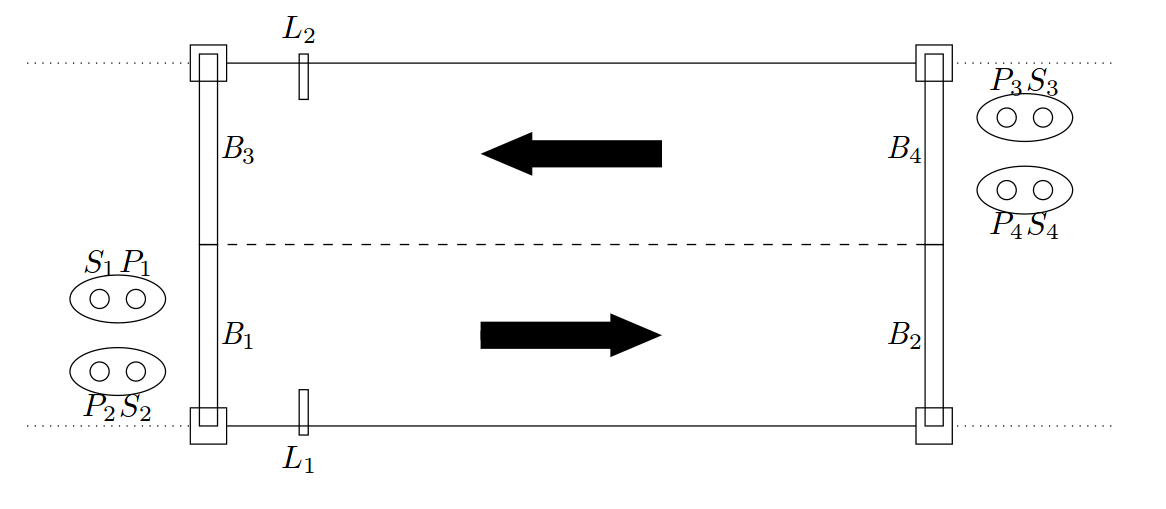
\includegraphics[width=1\textwidth]{sketch.png}
\caption{A situational sketch of the model and its components}
\label{fig:model}
\end{figure}

Our model also includes several sensors that will validate the preconditions that are required for our chain of actions. These sensors and their concurring sequence of actions are displayed in figure \ref{fig:sequence}. Using this chain of actions the global set of requirement was made. 


%--------------- Image of the sequence ------------
\begin{figure}[!h]
\centering
\includegraphics[width=0.5\textwidth]{model.pdf}
\caption{The sequence of actions in our model and the supporting sensors}
\label{fig:sequence}
\end{figure}
